\documentclass{article}%
\usepackage{amsmath}
\usepackage{amsfonts}
\usepackage{amssymb}
\usepackage{graphicx}
\usepackage{tikz}
\usepackage{xcolor}
\usepackage{hyperref}%
\setcounter{MaxMatrixCols}{30}
%TCIDATA{OutputFilter=late$x2$.dll}
%TCIDATA{Version=5.00.0.2552}
%TCIDATA{CSTFile=40 LaTeX article.cst}
%TCIDATA{Created=Thursday, August 21, 2008 14:03:59}
%TCIDATA{LastRevised=Wednesday, October 01, 2014 12:46:33}
%TCIDATA{<META NAME="GraphicsSave" CONTENT="32">}
%TCIDATA{<META NAME="SaveForMode" CONTENT="1">}
%TCIDATA{<META NAME="DocumentShell" CONTENT="Standard LaTeX\Blank - Standard LaTeX Article">}
%TCIDATA{Language=American English}
\newtheorem{theorem}{Theorem}
\newtheorem{acknowledgement}[theorem]{Acknowledgement}
\newtheorem{algorithm}[theorem]{Algorithm}
\newtheorem{axiom}[theorem]{Axiom}
\newtheorem{case}[theorem]{Case}
\newtheorem{claim}[theorem]{Claim}
\newtheorem{conclusion}[theorem]{Conclusion}
\newtheorem{condition}[theorem]{Condition}
\newtheorem{conjecture}[theorem]{Conjecture}
\newtheorem{corollary}[theorem]{Corollary}
\newtheorem{criterion}[theorem]{Criterion}
\newtheorem{definition}[theorem]{Definition}
\newtheorem{example}[theorem]{Example}
\newtheorem{exercise}[theorem]{Exercise}
\newtheorem{lemma}[theorem]{Lemma}
\newtheorem{notation}[theorem]{Notation}
\newtheorem{problem}[theorem]{Problem}
\newtheorem{proposition}[theorem]{Proposition}
\newtheorem{remark}[theorem]{Remark}
\newtheorem{solution}[theorem]{Solution}
\newtheorem{summary}[theorem]{Summary}
\newenvironment{proof}[1][Proof]{\noindent\textbf{#1.} }{\ \rule{0.5em}{0.5em}}

\usepackage{fancyhdr}
\setlength\headheight{26pt}
\pagestyle{fancy}
\lhead{{\footnotesize CSc 483 Final Exam - Study Guide}}
\rhead{{\footnotesize Christopher Chapline}}
\begin{document}
\section*{Vector Space Model}
\subsection*{Feast or Famine}
Feast or famine refers to the phenomenon where boolean retrieval models tend to retrieve either (1) A lot of results; or, (2) few results
\subsection*{Jaccard Coefficient}\\


$\textrm{Jaccard} = \frac{|A \bigcap B|}{|A \bigcup B|}, A \neq \emptyset , B \neq \emptyset$\\
\\
The Jaccard Coefficient measures the overlap between two sets, $A$ and $B$. In the context of information retrieval, it ignores term frequency
and does not normalize the length of individual documents.
\subsection*{TF-IDF}
$w_{t,d} = $
$\color{red} (1 + log(tf_{t,d}))$
$\cdot$
$\color{blue} log \left( \frac{N}{df_t} \right)$\\
\\
\textcolor{red}{tf-weighting}: The number of times that the term $t$ occurs in the document $d$.\\
\\
\textcolor{blue}{idf-weighting}: Measures the "informativeness" of the term $t$.

\subsection*{Vector Space Model}
Represents each document as a vector $v \in \mathbb{R}^{|V|}$ where $v$ is composed of $tf-idf$ weights. This means the document collection
is a real-valued vector space of $|V|$ dimensions. Terms represent axes in this space, documents are points or vectors.\\
\\
In this space, we can rank queries based on how close they are to the query.
\subsection*{Cosine Similarity}
We will rank documents according to their distance from the query in the vector space. To do this, we will rank them according to
$cosine(\vec{q}, \vec{d})$. We will normalize the lengths of the documents by dividing each component in each vector by the vector's
length.\\

$cos(\vec{q}, \vec{d}) = sim(\vec{q}, \vec{d}) = \frac{\vec{q} \cdot \vec{d}}{|\vec{q} \cdot \vec{d}|}
= \frac{\sum\limits_{i = 1}^{|V|}q_id_i}{\sqrt{\sum\limits_{i = 1}^{|V|}q_i^2 \sum\limits_{i = 1}^{|V|}d_i^2}}
$

\subsection*{Different Ways of Encoding}
\begin{tabular}{| l | l | l |}
    \hline
    Term Frequency                      & Document Frequency                & Normalization \\ \hline
    n (natural) $tf_{t,d}$              & n (no) 1                          & n (none) 1 \\
    l (logarithm) $1 + log(tf_{t,d})$   & t (idf) $log(\frac{N}{df_t}$      & c (cosine) $\frac{1}{\sqrt{w_1^2 + w_2^2 + \dots + w_M^2}}$ \\
    a (augmented) $0.5 + \frac{0.5 \cdot tf_{t,d}}{max_t(tf_{t,d})}$ & p (prob idf) $max{0, log \frac{N - df_t}{df_t}}$ & u (pivoted unique) $\frac{1}{u}$ \\
    b (boolean) \[ \begin{cases} 1 & if $tf_{t,d} > 0$ \\ 0 & otherwise \end{cases} \] & & b (byte size) $\frac{1}{CharLength^\alpha}, \alpha < 1$ \\
    L (log avg) $\frac{1 + log(tf_{t,d})}{1 + log(ave_{t \in d}(tf_{t,d}))}$ & & \\
    \hline
\end{tabular}
\section*{Complete Search System}
\subsection*{Exact Top K Retrieval using Min-Heap}
To process a new document d′ with score s′:\\

Get current minimum hm of heap (O(1)) \\

If $s\prime \leq hm$ skip to next document \\

If $s\prime > hm$ heap-delete-root $(O(log k))$ \\

Heap-add $d′/s′ (O(log k))$
\subsection*{Inexact Top K retrieval}
\begin{itemize}
    \item Order documents based on query-independent model (like PageRank)
    \item Primarily consider query terms with high $idf$ values
    \item Cluster Pruning (see figure 1)
\end{itemize}
\begin{figure}[h]
    \caption{Cluster pruning to retrieve top K results}
    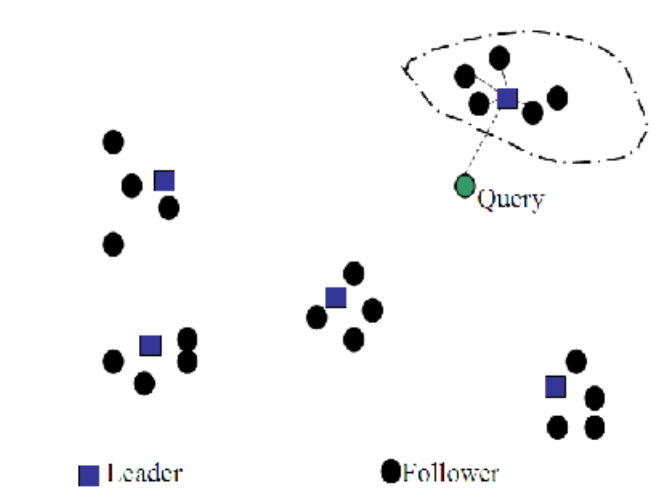
\includegraphics[scale=.5]{ClusterPruning.png}
    \centering
\end{figure}
\section*{Evaluation}
\subsection*{Unranked evaluation}
\textbf{Precision (P)}: The fraction of retrieved documents that are relevant \\
\\
\textbf{Recall (R)}: The fraction of relevant documents that are retrieved \\
\\
\textbf{F Score}: Allows a trade off between precision and recall \\

$F = \frac{1}{\alpha \frac{1}{P} + (1 - \alpha)\frac{1}{R}} = \frac{(\beta^2 + 1) PR}{\beta^2P + R}
\textrm{ where } \beta^2 = \frac{1 - \alpha}{\alpha}$ \\
\\
and where\\

$\alpha \in [0, 1] \textrm{ and } \beta^2 \in [0, \infty]$\\
\\
Most frequently, \textbf{balanced F} is used where $\alpha = 0.5$ and $\beta = 1$
\subsection*{Accuracy}
In IR, striving for accuracy would frequently result in nothing being returned. Instead, we want
to return \textit{something}, even if what is returned isn't necessarily accurate.
\subsection*{Ranked evaluation}
\textbf{Precision-Recall Curve}: Each point corresponds to a result for the top $k$ ranked hits\\
\\
\textbf{Mean Average Precision (MAP)}: Roughly the area under the precision-recall curve\\

$MAP(Q) = \frac{1}{|Q|} = \sum\limits_{j=1}^{|Q|}\frac{1}{m_j} \sum\limits_{k = 1}^{m_j} \textrm{Precision}(R_{jk})$\\
\\
where\\

$m_j$ - number of relevant documents for query $j$.\\

$R_{jk}$ - number of documents until the relevant document $d_k$ for query $j$.\\
\\
\textbf{Mean Reciprocal Rank (MRR)}: $MRR(Q) = \frac{1}{|Q|} \sum\limits_{j = 1}^{|Q|}\frac{1}{\textrm{rank}_j}$
where $\textrm{rank}_j$ is the position of top correct answer for query $j$.
\subsection*{Inter-Annotator Agreement}
\textbf{Kappa measure}: Measures how much judges agree or disagree\\

$\kappa = \frac{P(A) - P(E)}{1 - P(E)}$\\
\\
where\\

$P(A)$ = proportion of judges which agree \\

$P(E)$ = agreement we would get by chance\\
\\
For these measures, $\kappa \in [\frac{2}{3}, 1]$ is seen as acceptable
\subsection*{Real-world evaluations}
\textbf{A/B testing}: Testing a feature by splitting a portion of your user base and introducing the
feature to that small portion. Evaluate how well the new feature is recieved by the portion of the
userbase with automatic evaluation technology.
\subsection*{Result Summaries}
\textbf{Static Summaries}: Summary is always the same regardless of the query (i.e first 50 words, etc.) \\
\\
\textbf{Dynamic Summaries}: Query dependent. Attempt to explain why the document was retrieved for the query
\subsection*{Criteria for good dynamic summaries}
\begin{itemize}
    \item Maximally informative for query
    \item Self-contained, easy to read
    \item Short enough, shouldn't take up real estate
\end{itemize}
\section*{Relevance Feedback \& Query Expansion}
\subsection*{Centroid}
The centroid is the center of mass for a set of points. Since we represent documents as points in a
high-dimensional space, we can compute the centroid of a collection of documents.\\

$\vec{\mu}(D) = \frac{1}{|D|} \sum\limits_{d \in D}\vec{v}(d)$\\
\\
where $D$ is the set of documents and $\vec{v}(d)$ is the vector for the document $d$.
\subsection*{Rocchio algorithm}
\begin{figure}[h]
    \caption{An illustration of the Rocchio algorithm}
    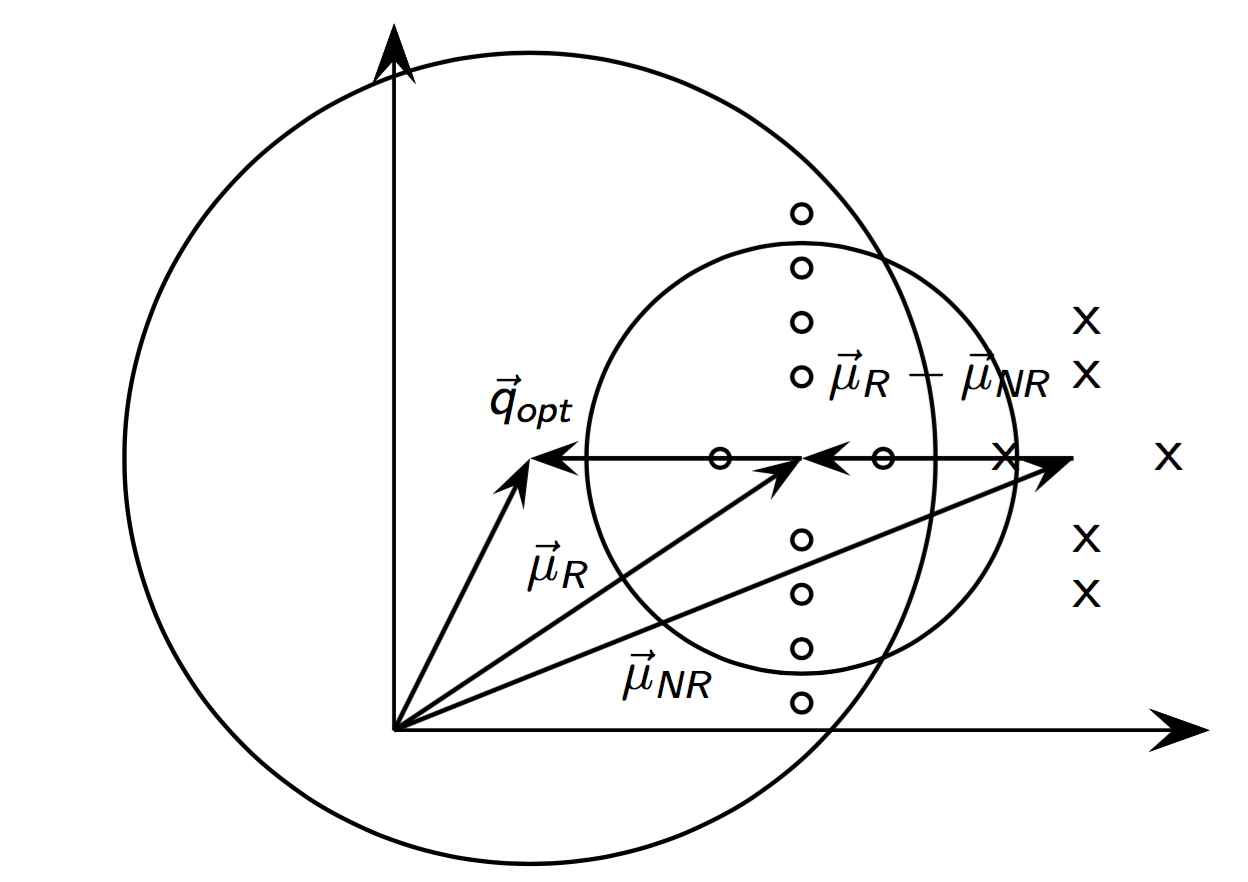
\includegraphics[scale=.3]{Rocchio.png}
    \centering
\end{figure}
Implements relevance feedback in the vector space model. Rocchio chooses the query $\vec{q}_{opt}$
that maximizes: \\

$\vec{q}_{opt} = \textrm{arg}_{\vec{q}} \textrm{max} [sim(\vec{q}, \mu(D_r)) - sim(\vec{q}, \mu(D_{nr}))]$ \\
\\
where $D_r$ is the set of relevant documents and $D_{nr}$ is the set of non-relevant documents.\\
\vspace{2mm}\\
The vector $\vec{q}_{opt}$ is the vector that separates relevant and non-relevant documents. With some additional
assuptions, we can rewrite this as: \\

$\vec{q}_{opt} = \mu(D_r) + [\mu(D_r) - \mu(D_{nr})]$\\
\\
In practice, the SMART algorithm is used: \\

$\vec{q}_m = \alpha \vec{q_0} + \beta \mu(D_r) - \gamma \mu(D_{nr})
= \alpha \vec{q_0} + \frac{\beta}{|D_r|} \sum\limits_{\vec{d_j} \in D_r}\vec{d_j} - \frac{\gamma}{|D_{nr}|} \sum\limits_{\vec{d_j} \in D_{nr}} \vec{d_j}$ \\
\\
where
\begin{itemize}
    \item $\vec{q_m}$ - Modified query vector
    \item $\vec{q_0}$ - Original query vector
    \item $D_r$ and $D_{nr}$ sets of known relevant and non-relevant documents
    \item $\alpha$, $\beta$, and $\gamma$ are weights
\end{itemize}
\subsection*{Query Expansion Using Global Resources}
Some examples of global resources which can be used for query expansion:
\begin{itemize}
    \item Manual thesaurus maintained by editors
    \item Automatically derived thesaurus (co-occurence statistics)
    \item Query-equivalence based on query log mining
\end{itemize}
\subsection*{Query expansion at search engines}
Primary source of query expansion in search engines comes from mining the query logs from those search engines. If queries frequently occur
within immediate proximity of one another, then you can begin to draw equivalence between those two queries.
\section*{Probabilistic Information Retrieval}
\subsection*{Basic probability theory:}
\textbf{Conditional Probability}: $P(A | B) = \frac{P(A \bigcap B)}{P(B)}$ \\
\\
\textbf{Chain Rule}: $P(A \bigcap B) = P(A | B) \cdot P(B)$ \\
\\
\textbf{Bayes' Rule}: $P(A | B) = \frac{P(A \bigcap B)}{P(B)} = \frac{P(A)P(B | A)}{P(B)}$ \\
\\
\textbf{Law of Total Probability}: $P(B) = P(A) P(B | A) + P(\overline{A}) P(B | \overline{A})$ \\
\\
\textbf{Odds}: $O(A) = \frac{P(A)}{P(\overline{A})} = \frac{P(A)}{1 - P(A)}$ \\
\\
\textbf{Independent Events}: $A$ is independent of $B$ if $P(A | B) = P(A)$.
\subsection*{Probability Ranking Principle}
If the retrieved documents (with respect to a query) are ranked decreasingly on their probability of
relevance, then the effectiveness of the system will be the best that is obtainable

\subsection*{Binary independence model}
A document $d$ is represented as a vector $\vec{x} = (\vec{x}_1, \ldots, \vec{x}_M)$ where $x_t = 1$ if $t$ occurs in $d$ and $x_t = 0$
otherwise. We make the assumption of independence between terms, which means that there is no association between terms. Theoretically,
this is false, but it works in practice.\\
\\
\begin{tabular}{| l l | l l | l |}
    \hline
                    & document      & relevent ($R = 1$)    & nonrelevant ($R = 0$) & Total \\
    \hline
    Term present    & $x_t = 1$     & $s$                   & $df_t - s$                & $df_t$ \\
    Term absent     & $x_t = 0$     & $S - s$               & $(N - df_t) - (S - s)$    & $N - df_t$ \\
    \hline
                    & Total         & S                     & N - S                     & N \\
    \hline
\end{tabular}\\
\\
$p_t = s/S$ \hfill $u_t = (df_t - s) / (N - S)$\\
\\
We rank documents using log odds ratios for terms in the query $c_t$: \\

$c_t = log \frac{p_t (1 - u_t)}{u_t (1 - p_t)} = log \frac{p_t}{1 - p_t} - log \frac{u_t}{1 - u_t}$\\
\\
The result for $c_t$ can be interpreted like so:
\begin{itemize}
    \item $c_t = 0$ term has equal odds of appearing in relevant and non-relevant documents
    \item $c_t > 0$ term has higher odds to appear in relevant documents
    \item $c_t < 0$ term has higher odds to appear in nonrelevant documents
\end{itemize}
how to derive the ranking function for terms; the formula for ct, with smoothing; BIM after simplifying assumptions}
\subsection*{Okapi BM25}
Improve $idf$ term by factoring in term frequency and document length:\\

$RSV_d = \sum\limits_{t \in q} log \left[ \frac{N}{df_t} \right] \cdot \frac{(k_1 + 1) tf_{td}}{k_1 ((1 - b) + b \cdot (L_d /L_{ave})) + tf_{td}}$ \\
\\
where
\begin{itemize}
    \item $tf_{td}$: Term frequency in document $d$
    \item $L_d$: and $L_{ave}$: Length of $d$ and average document length respectively
    \item $k_1$: Controlling document term frequency scaling $k_1 > 0$
    \item $b$: Controlling scaling by document length $b \in [0, 1]$
\end{itemize}

\section*{Language Models}
\subsection*{Smoothed LM Ranking}
For a query $q$, we compute $P(q | d)$ using the following equation: \\

$P(q | d) \propto \prod\limits_{1 \leq k \leq |q|}(\lambda P(t_k | M_d) + (1 - \lambda) P(t_k | M_c)$ \\
\\
where \\

$P(t | M_d) = \frac{tf_{t,d}}{|d|}$ \\

$P(t | M_c) = \frac{cf_t}{T}$
\subsection*{N-Gram Language Models}
These models are used in applications where the independence assumption made in language models is impossible, such as text prediction systems.
\section*{Text Classification \& Naive Bayes}
\subsection*{Why Text Classification}
Text classification is used for things like automatic language detection, spam detection, sentiment detection, etc.
\subsection*{How to compute P(c $\vert$ d), smoothing}
We compute $P(c | d)$ as: \\

$P(c | d) \propto P(c) \prod \limits_{1 \leq k \leq n_d} P(t_k | c)$\\
\\
where $n_d$ is the length of the document, $P(t_k | c)$ is a measure of how much evidence $t_k$ contributed that $c$ is the correct class,
and $P(c)$ is the prior probability of $c$.\\
\vspace{2mm}\\
To prevent floating point underflow, what is usually computed in practice is:\\

$P(c | d) \propto logP(c) + \prod \limits_{1 \leq k \leq n_d} log P(t_k | c)$
\subsection*{Multinomial vs. Bernoulli}
The Bernoulli model estimates  $P(t | c)$ as the fraction of documents of class $c$ that contain term $t$.\\
\\
In contrast, the multinomial model estimates  $P(t | c)$ as the fraction of tokens or fraction of positions in documents of class $c$ that contain term $t$
\subsection*{Naive Bayes Pitfalls (3)}
\begin{itemize}
    \item Underflow: Not using log probabilities
    \item Zero Counts: Not smoothing
    \item Not doing feature selection
\end{itemize}
\subsection*{Naive Bayes Assumptions (2)}
\begin{itemize}
    \item Conditional Independence Assumption: We assume that the probability of observing the conjunction of attributes is equal
        to the product of the individual probabilities $P(X_k = t_k|c)$.
    \item $P(X_{k1} = t | c) = P(X_{k2} = t | c)$. The probability of generating a term in the first position is equal to the
        probability of generating that term in the last position
\end{itemize}\\
\\
The combination of these assumption amount of \textbf{bag of words}.
\subsection*{Evaluating classification}
Macroaveraging:
\begin{enumerate}
    \item Compute $F_1$ for $C$ classes
    \item Average these $C$ numbers
\end{itemize}\\
\\
Microaveraging:
\begin{enumerate}
    \item Compute $TP$, $FP$, and $FN$ for each of the $C$ classes
    \item Sum these $C$ numbers
    \item Compute $F_1$ for aggregate $TP$, $FP$, and $FN$.
\end{itemize}

\subsection*{Feature selection}
There are several different ways of picking features:
\begin{itemize}
    \item Frequency: Select the most frequent terms
    \item Mutual Information: Select the terms with the highest mutual information
    \item Chi-Squared: Measure how much expected counts $E$ and observed counts $N$ deviate from each other
\end{itemize}
\section*{Vector Space Classification}
\subsection*{Rocchio}
Basic idea of Rocchio:
\begin{enumerate}
    \item Compute centroid for each class
    \item Assign each test document to the class of its closest centroid
\end{itemize}\\
\\
In most cases, Rocchio performs worse than Naive Bayes' because it cannot handle nonconvex, multimodal
classes correctly (see figure 3):
\begin{figure}[h]
    \caption{An example of nonconvex, multimodal classes}
    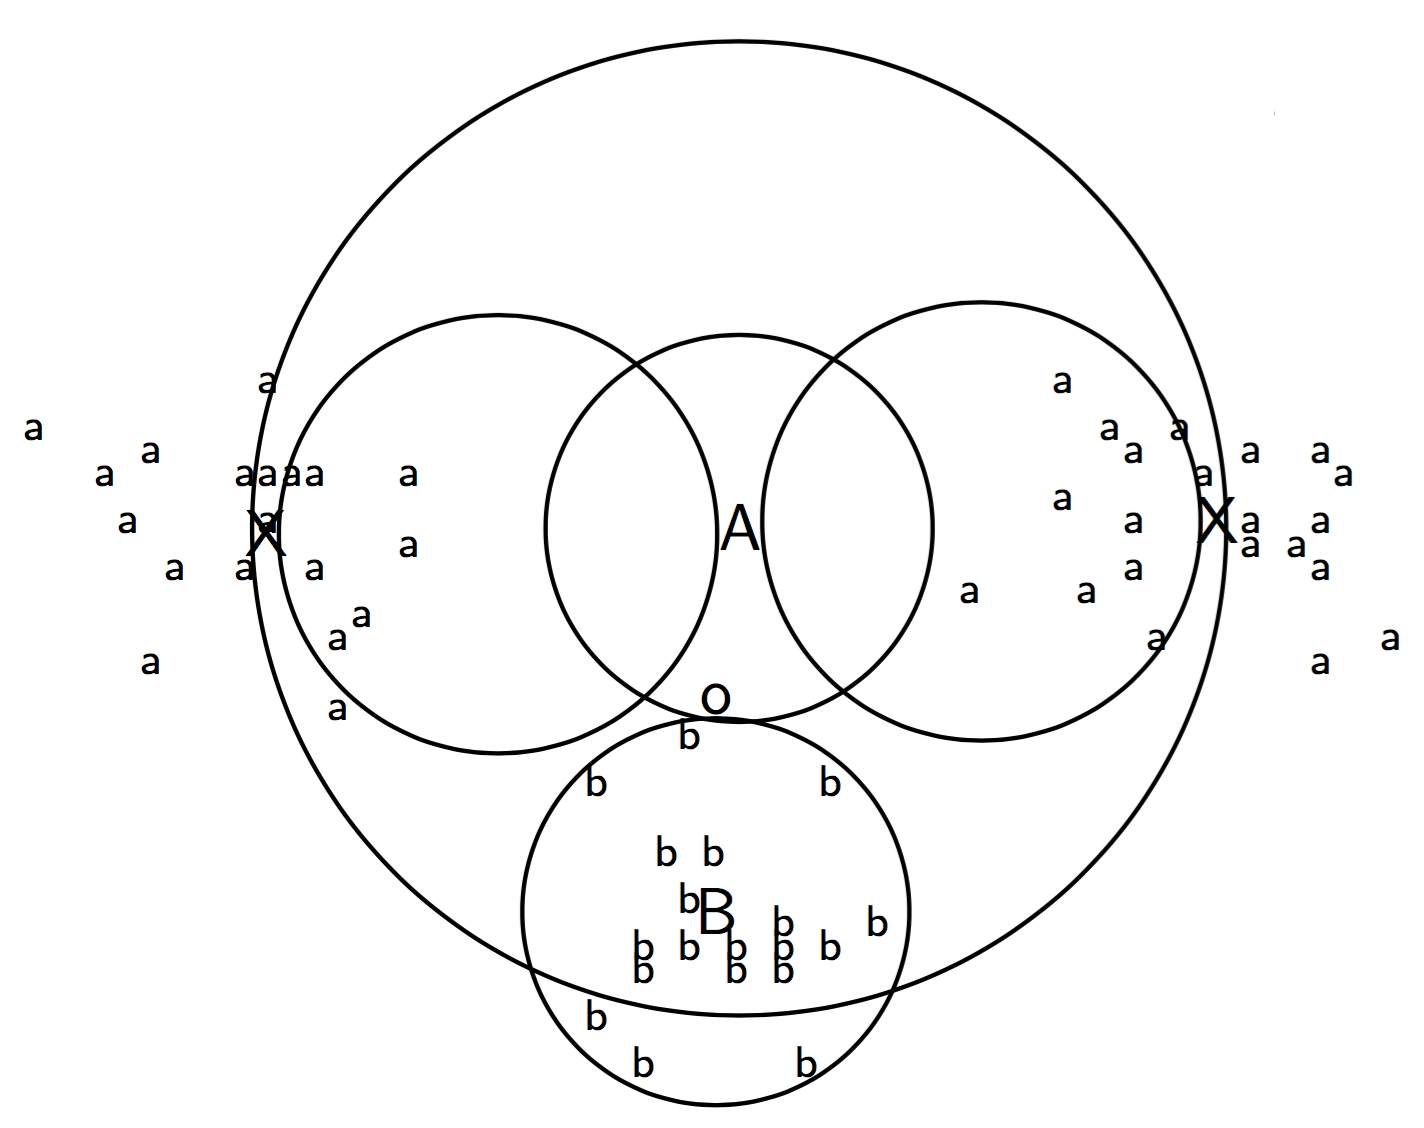
\includegraphics[scale=.3]{nonconvex.png}
    \centering
\end{figure}
\subsection*{K Nearest Neighbors}
Assign the document $d$ to the most popular class amongst it's $k$ nearest neighbors. In probabilistic IR,
you can represent this as finding the class $c$ that maximizes $P(d | c$ for the document $d$.\\
\\
The time complexity to train kNN is $\Theta(|\mathbb{D}| L_{ave})$. For testing, its time complexity is
$\Theta(L_a + |\mathbb{D}|M_{ave}M_a) = \Theta(|\mathbb{D}| M_{ave}M_a)$.
\section*{Flat Clustering}
\subsection*{Classification vs. Clustering}
Classification is a form of supervised learning. It requires a series of training data which determine the
kinds of classes that documents can be classified into. Clustering is a form of unsupervised learning where
clusters are \textit{inferred from the data} without human input.
\subsection*{Applications of Clustering in IR}
\begin{itemize}
    \item Search results to provide more information to the user
    \item Clustering collections for exploratory browsing
    \item Cluster-based retrieval for higher efficiency/faster searching
\end{itemize}
\subsection*{K-means}
K-means is an algorithm designed to find a clustering for a collection of documents. It does this by computing
centroids and attempting to minimize the average squared distance from the centroid.\\

$\mu(\omega) = \frac{1}{\omega} \sum \limits_{\vec{x} \in \omega} \vec{x}$ \hfill (Centroid definition for a cluster $\omega$)\\
\\
The process iterates over two steps:
\begin{itemize}
    \item \textbf{Reassignment}: Assign each vector to its closest centroid
    \item \textbf{Recomputation}: Recompute each centroid as the average of the vectors that were assigned to it in reassignment
\end{itemize}\\
\\
This is guarenteed to converge on the optimal clustering:
\begin{enumerate}
    \item Let $RSS$ be the sum of all squared distances between document vectors and their closest centroids
    \item $RSS$ decreases during each reassignment step because each vector is moved to a closer centroid
    \item $RSS$ decreases during each recomputation step
    \item Since there are only a finite number of clusterings, it will eventually converge on the optimal one
\end{itemize}

\subsection*{K-means++}
\subsection*{Clustering evaluation}
purity, Rand index, F measure
\subsection*{Number of clusters}
\section*{Link Analysis \& Page Rank}
\subsection*{Anchor text}
what it is, how to index, how to search
\subsection*{Google bombs}
\subsection*{PageRank}
random walk problem\\
\\
how to construct the probability matrix\\
\\
teleportation probability\\
\\
how to compute the steady state vector using the power method\\
\\
issues\\
\\

\end{document}
